\documentclass[a4paper,11pt]{article}
\usepackage{a4wide}
\usepackage{fullpage}
\usepackage[utf8x]{inputenc}
%\usepackage[slovene]{babel}
%\selectlanguage{slovene}
\usepackage[toc,page]{appendix}
\usepackage[pdftex]{graphicx} % za slike
\usepackage{setspace}
\usepackage{color}
\definecolor{light-gray}{gray}{0.95}
\usepackage{listings} 

\begin{document}
\chapter{Modeliranje TCP/IP omrežij}
%\chapterauthor{Matevž Ogrinc, Robert Modic, Andreja Kovačič}

\section{Gradniki za realizacijo IPv4 omrežij}
	\begin{itemize}
		\item\textit{IPv4}: glavni modul, ki implementira IP protokol(RFC 791). Modul izvaja enkapsulacijo, dekapsulacijo, fragmentacijo in defragmentacijo in usmerjanje IP datagramov. Prispeli paketi se posredujejo v ARP modul. Privzeta predpostavka modula je, da se vsi paketi obravnavajo enako dolgo, brez prioritet. Za drugačne nastavitve je treba spremeniti implementacijo.
		\item\textit{IPv4RoutingTable}: pomožni modul, ki skrbi za usmerjevalne tabele vozlišč. Vsak gostitelj in usmerjevalki vsebuje eno kopijo. Modulu IPv4 dostavlja podatke o najboljših poteh, posodabljajo pa ga daemoni RIP, OSPF, Manet in drugih protokolov. Modul nima vrat, vsa komunikacija z njim poteka skozi klice funkcije (predvsem read in update). Ko je na voljo več poti za dan naslov, se upošteva pot:
		z najdaljšim ujemanjem naslova,z najbolj specifično multicast skupino, z najmanjšo metriko (ceno poti).
		\item\textit{ICMP}: modul generira ICMP(RFC 792) pakete, podpira echo aplikacije. ICMP protokol se uporablja za spetno javljnje napak in diagnostiko. Ker uporablja protokol IP, spada med transportne protokole, vendar se za razliko od TCP/UDP protokolov ne uporablja za prenos uporabnikovih podatkov.
		\item\textit{ARP}: izvaja dinamično prevajanje med lokalnimi naslovi(tipično IP) in strojnimi naslovi(MAC), implementira RFC 826. Inet-ova implementacija podpira samo preslikavo IP-MAC.
		\item\textit{IGMPv2}: Modul generira in procesira multicast sporočila o članstvu odjemalcev v multicast skupine. Podatke posreduje usmerjevalnikom v omrežju. Ko se vmesnik gostitelja želi včlaniti v skupino, pošlje IGMP poročilo vmesniku multicast usmerjevalnika, ta ga obdela in posodobi tabelo naslovnikov multicast sporočil. Podoben postopek je ob izstopu gostitelja iz skupine. 
	\end{itemize}


Moduli so sestavljeni v \textit{IPv4NetworkLayer}, ki predstavlja celotno omrežno plast. Ima vrata za TCP, UDP, SCTP, RSVP in druge protokole.  Nanj se lahko povežejo omrežni vmesniki: Ethernet, PPP, Wlan ali drugi zunanji vmesniki. Modul se uporablja za gradnjo gostiteljev(hosts) in usmerjevalnikov (routers).
\pagebreak
\setlength{\parindent}{0pt}
\section{Zgledi IPv4 omrežij v OMNeT++}
\subsection{Primer 1 - Multicast}

\large \bf Opis omrežja in gradnikov\par
\normalfont \normalsize 
\setlength{\parindent}{10pt}
Multicast omrežje je sestavljeno iz štirih usmerjevalnikov (tipa Router) in šestih odjemalcev (tipa StandardHost). Prikazuje pretok paketov, ki so namenjeni enemu naslovniku torej unicast hkrati pa tudi večim naslovnikom, ki spadajo v skupine ali multicast skupine. Paketi so duplicirani v usmerjevalniku samo v primeru kadar obstajajo poslušalci v njegovem omrežju. Torej usmerjevalnik vnaprej pozna poslušalce določenih multicast skupin. To dosežemo z uporabo protokol v našem primeru IGMPv2, saj IPv4 takega delovanja ne podpira sam po sebi.
\begin{figure}[h]
	\centering
	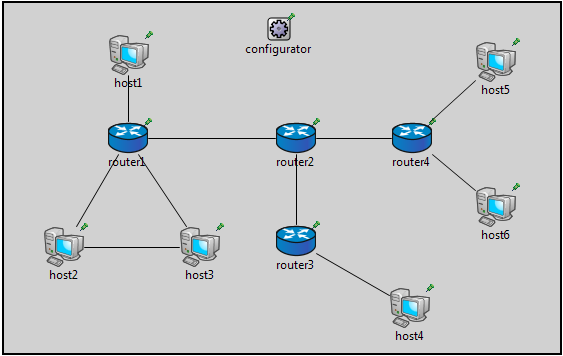
\includegraphics[width=\textwidth]{Multicast.png}
	\caption{Omrežje Multicast in njegovi gradniki}
	\label{Multicast}	
\end{figure}\par
\setlength{\parindent}{0pt}
\large\bf Podrobna analiza\par
\normalfont \normalsize 
\setlength{\parindent}{10pt}
Ob zagonu simulacije opazimo pakete tipa IGMPv2Query iz tako imenovanega glavnega usmerjevalnika v našem primer je to usmerjevalnik2 (router2), ki predstavlja povpraševanje po obstoječih poslušalcev multicast naslovov, nato kot odgovor iz vsakega od vozlišč opazimo paket IGMPv2Report. Ob prejemu tega paketa lahko glavni usmerjevalnik ustvari multicast tabelo, saj mu pove ali obstaja poslušalec za nek multicast naslov. Tabela usmerjevalniku pove, ob prispelem multicast paketu, ali naj paket pošlje naprej ali ne in kam. Ob končani poizvedbi se prične normalni pretok multicast paketov do odjemalcev oz poslušalcev. Če pogledamo glavni usmerjevalnik opazimo, da vsebuje njegova multicast tabela tri multicast skupine: 
\begin{enumerate}
	\item (127.0.0.x) s poslušalci host1,host2 in host3 ter usmerjevalnikom1
	\item (127.0.1.x) s poslušalcem host4 in usmerjevalnikom3
	\item (127.0.2.x) za poslušalca host5, host6 in usmerjavalnikom4
\end{enumerate} 
\subsection{Primer 2 - Flatnet}\par
\large \bf Opis omrežja in gradnikov\par
\normalfont \normalsize 
Omrežje je sestavljeno iz enega strežnika, 57 usmerjevalnikov in dveh odjemalcev. Namen tega omrežja je prikazati avtomatsko sestavo routing tabele in dodeljevanje IP naslovov, hkrati pa tudi prikaže proces three-way handshake-a med odjemalcem in strežnikom za prenos podatkov. Omrežje ima dve vrsti povezovanja, preko Ethernet kabla in optike. Zaradi velike količine usmerjevalnikov bomo omrežje ponazorili z spodnjo sliko.
\begin{figure}[h]
	\centering
	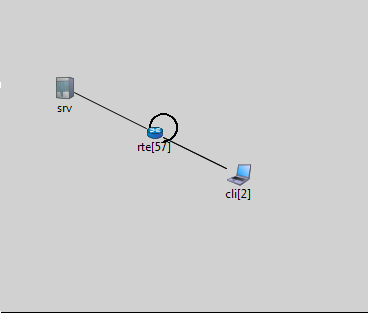
\includegraphics{FlatNet.png}
	\caption{Omrežje FlatNet in njegovi gradniki}
	\label{flatNet}	
\end{figure} 

\setlength{\parindent}{0pt}
\large\bf Analiza flatnet\par
\setlength{\parindent}{10pt}
\normalfont \normalsize 
Ob zagonu simulacije se pošljejo iz odjemalca SYN paketi oz Synchronization packets. Paketi potujejo po usmerjevalni tabeli od usmerjevalnikov do strežnika kjer nato strežnik odgovori z SYN-ACK oz acknowledge paketi, ki potujejo po istih usmerjevalnikih nazaj. Ob prejemu SYN-ACK paketa odjemalec odgovori z istim SYN-ACK paketom. SYN paketi se uporabljajo za vzpostavitev three-way handshake procesa v TCP-ju. To se zgodi kadar odjemalec želi pošiljati drugemu odjemalcu podatke. Po three-way handshake procesu odjemalec začne pošiljati podatke v obliki TCP segmentov. Ob prejemu teh se strežnik odzove z ACK oz acknowledge paketi. Celoten proces se zgodi za oba odjemalca. S to razliko da eden uporablja ethernet, drugi pa optično povezavo. Omrežje deluje zato, ker ima avtomatsko dodeljevanje IPv4 naslovov in avtomatsko kreirane usmerjevalne tabele, da lahko paketi pridejo do cilja.

\pagebreak
\subsection{Primer 3 - Bulktransfer}\par
\large \bf Opis omrežja in gradnikov\par
\normalfont \normalsize 
Omrežje je sestavljeno iz enega usmerjevalnika, tremi odjemalci in enim strežnikom. Namen je prikazati uporabo TCP client/Server modele za prenos večjih datotek ali "Bulktransfer". Dva odjemalca sta povezana z strežnikom preko usmerjevalnika, eden je pa povezan direktno, kot je razvidno na spodnji sliki.
\begin{figure}[h]
	\centering
	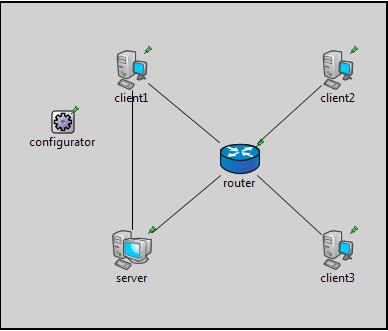
\includegraphics[width=\textwidth]{BulkTransfer.png}
	\caption{Omrežje bulktransfer in njegovi gradniki}
	\label{bulkTransfer}	
\end{figure}

\setlength{\parindent}{0pt}
\large\bf Analiza bulktransfer\par
\setlength{\parindent}{10pt}
\normalfont \normalsize
Ob zagonu simulacije se iz odjemalca(client 1) pošlje Syn paket za three-way handshake s strežnikom. Ob istem času pa iz odjemalca (client 2 in client 3) prihaja isti SYN paket najprej za usmerjevalnik nato usmerjevalnik SYN paket pošlje do strežnika. Vsi trije odjemalci prejmejo SYN-ACK pakete in opravijo three-way handshake z strežnikom. Nato odjemalci pošljejo na strežnik maksimalno velike pakete ter jih hkrati od strežnika tudi prejemajo. Ob prejemu TCP segmenta pošljejo strežniku ali strežnik njim ACK. potrditev, da so segment prejeli. Za prenos moramo večje datoteke razdeliti na segmente in jih po delih pošiljati do strežnika, kar ta simulacija tudi ponazarja.

\pagebreak

\section{Načrtovanje omrežij}\par
\large \bf Opis \par
\normalfont \normalsize
Omrežje je sestavljeno iz treh serverjev in osmih odjemalcev. Trije usmerjevalniki (router 2,5,6) predstavljajo hrbtenico omrežja, nihče od odjelamcev ali serverjev ni neposredno povezan nanje. Med njimi so zelo hitre optične povezave, sicer ima omrežje bakrene kable, ki dosegajo manjše hitrosti prenosa. 
\subsection{Omrežje z optično hrbtenico}

\begin{figure}[h]
	\centering
	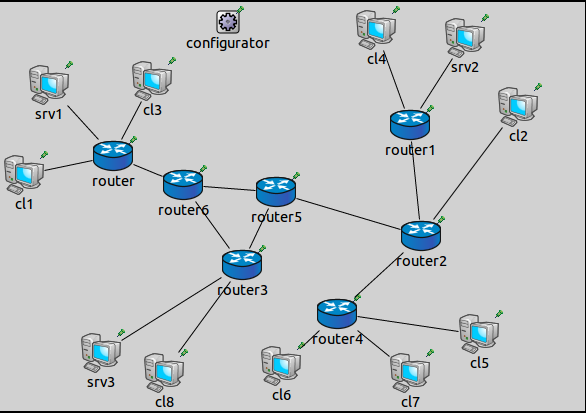
\includegraphics[width=\textwidth]{omrHrbtenica.png}
	\caption{Omrežje z optično hrbtenico}
	\label{bulkTransfer}	
\end{figure}
\end{document}